\documentclass[conference]{IEEEtran}
\IEEEoverridecommandlockouts
% The preceding line is only needed to identify funding in the first footnote. If that is unneeded, please comment it out.
\usepackage{cite}
\usepackage{amsmath,amssymb,amsfonts}
\usepackage{algorithmic}
\usepackage{graphicx}
\usepackage{textcomp}
\def\BibTeX{{\rm B\kern-.05em{\sc i\kern-.025em b}\kern-.08em
    T\kern-.1667em\lower.7ex\hbox{E}\kern-.125emX}}
\begin{document}

\title{The acceleration of public--key cryptanalysis methods using Xilinx Zynq-7000
%Akcelerace metod kryptoanalýzy asymetrických kryptosystémů %Paper Title*\\
%{\footnotesize \textsuperscript{*}Note: Sub-titles are not captured in Xplore and
%should not be used}
%\thanks{Identify applicable funding agency here. If none, delete this.}
}

\author{
\IEEEauthorblockN{David Salac}
\IEEEauthorblockA{\textit{Institute of Information Technology and Electronics} \\
\textit{Technical university of Liberec}\\
Liberec, Czech republic \\
david.salac@tul.cz}
\and
\IEEEauthorblockN{Martin Rozkovec}
\IEEEauthorblockA{\textit{Institute of Information Technology and Electronics} \\
\textit{Technical university of Liberec}\\
Liberec, Czech republic \\
martin.rozkovec@tul.cz}
}

\maketitle

\begin{abstract}
The Xilinx Zynq-7000 SoC provides new possibilities for increase of efficiency of cryptanalysis methods  for public--key systems such as RSA or Diffie--Hellman key exchange algorithm. These cryptosystems are based on the discrete logarithm and integer factorization problem. After brief introduction to numerical methods for solving of these problems there is an introduction to the distributed system that aims to solving of these problems. Distributed system consists of master nod that manage the distribution of the tasks and slave nods that computes one of the most time consuming part of the selected numerical methods called sieving. Afterward the slave nod is designed on Xilinx Zynq-7000 SoC consists of ARM processor for analyzing of the problem and some custom IP cores running on FPGA for increasing of the efficiency of algorithm. The capabilities of distributed system is also measured and analyzed afterward.
\end{abstract}

\begin{IEEEkeywords}
GNFS, FPGA, Quadratic Sieve, Zynq-7000, Index Calculus
\end{IEEEkeywords}

\section{Introduction}
Together with increasing computational potential of FPGA and new approach of designing of the specialized hardware there arise issue of security of public--key cryptosystems. This paper aims to aims to analyze the possibilities of Xilinx Zynq-7000 SoC in solving of integer factorization and discrete logarithm problem. It means it analyze its potential on implementation of cryptanalysis methods for solving of mentioned problems. 

\section{Security of public--key cryptosystems}
There are many ciphers and protocols in a branch of public--key cryptography. But only methods based on principle of simple integer factorization and discrete logarithm are relevant in this paper. 

\subsection{Integer factorization problem}
The example of cipher based on principle of integer factorization problem is RSA cryptosystem that use public key $n$ of format $n = pq$ for some large prime numbers $p$ and $q$ and some integer $e$ such that $e \nmid \varphi(n)$, where $\varphi(n)$ represents Euler's totient function \cite{delfs}. The security of this cipher is based on toughness of finding numbers $p$ and $q$ for given number $n$ that could be afterward used for computing of $\varphi(n)$ and the value of $d$. 

In general, integer factorization problem could be defined as searching for the decomposition of given positive integer $n$ to following format:
\begin{equation}
n = \prod_{i = 1}^r p_i^{a_i}
\end{equation}
where $p_i$ is a prime number and $a_i$ is a natural number (for each $i = 1,2,\cdots,r$).

There are no known effective algorithm for solving of this problem in polynomial time (excepting the Shor's algorithm for quantum computers). The best known algorithms for solving of the integer factorization problem for large integers are \cite{yan}:
\begin{itemize}
\item \textbf{Quadratic Sieve} -- for integers of size less than approximately $10^{100}$.
\item \textbf{General Number Field Sieve} -- for integers of size greater than approximately $10^{100}$.
\end{itemize}

\subsection{Discrete logarithm problem}
The security of public--key cryptosystems could also be based on discrete logarithm problem \cite{delfs}. Suppose that there is prime number $p$ and the primitive root mod $p$ -- integer $g$ and random number $a \in \mathbb{Z}_p$. Discrete logarithm problem is searching for the value of integer $k$ in following congruence:
\begin{equation} \label{eq:dlg}
g^k \equiv a \pmod{p}
\end{equation}
There is also no known effective algorithm (excepting Shor's algorithm for quantum computers) for doing such operation. Numerical methods for solving of this problem are usually based on combination of following methods \cite{yan}: 
\begin{itemize}
\item \textbf{Pohlig--Hellman algorithm} that could simplify the congruence \eqref{eq:dlg}.
\item \textbf{Index Calculus} that is the common method (and the most effective one) for solving of discrete logarithm problem.
\end{itemize}

The well-known public--key protocol based on this principle is Diffie--Hellman key exchange.

\subsection{The others approach in public--key cryptography}
There are also many others public--key cryptosystems based on different principles. Especially the elliptic curve cryptography is well known. Many quantum--resistant algorithms based on some NP--complete problems are also available. Numerical methods for cryptanalysis of this algorithms are not the subject of this paper.

\section{Effective approach in cryptanalysis}
The only way how to succeed in solving some real cryptanalysis integer factorization or discrete logarithm problem is to use some of the mentioned numerical methods and parallel approach for this purpose. The possibility of using the FPGA for accelerating of some parts of mentioned numerical methods is discussed bellow.

\subsection{Parallel approach in integer factorization problem}
Each of the currently used method for integer factorization is similar to (or based on) Dixon's Random Square Method. This method consists two steps, the first one is called sieving the other one is called matrix processing. Each of this steps could be distributed for many computational nods.

The sieving part of the algorithm consists of searching for some integers that are smooth over some factor base $F$ (that usually contains prime numbers, for example first $|F|$ prime numbers). The method tries to find a set of integers $x_i$ such that $\sqrt{n} < x_i < n$ and the value $(x_i^2 \mod n)$ is smooth over a set $F$. It means that there exists following decomposition:
\begin{equation} \label{eq:sieving}
x_i^2 \mod n = \prod_{ \substack{p_j \in F \\ e_{ij} \in \mathbb{Z}^+} } p_j^{e_{ij}}
\end{equation} 
Algorithm has to find at least $\left ( |F|+1 \right)$ of such integers $x_i$ \cite{yan}. This process could be easily distributed to as many nods as possible. Each nod just generate the random value $x_i$ and check the smoothness of $x_i$ over the factor base $F$. Others algorithms (especially General Number Field Sieve and Quadratic Sieve) have sieving part that is similar to the represented one. The sieving part of algorithm is usually the slower one and it is especially sensitive for selecting of the right value of method's parameters. 

The matrix processing part of algorithm consists of computing the null space of matrix of the exponents $e_{ij}$ found in step \eqref{eq:sieving} over finite $\mathbb{Z}_2$ field (because only the parity of exponents is relevant). Because of the sparsity of given matrix the block Lanczos algorithm could be used in this process as an effective algorithm \cite{lanczos}, \cite{hoang}. The size of matrix is about $10^6$ rows and cols in practice (for $n > 2^{512}$). The other method for computing of null space of sparse matrix is Wiedemann algorithm \cite{wiedemann} which could be distributed to many computational nods.

After the matrix processing part the values of integers $x$ and $y$ are found such that \cite{yan}:
\begin{equation}
x^2 \equiv y^2 \pmod{n} \hspace{10pt} \land \hspace{10pt} x \not\equiv \pm y \pmod{n}
\end{equation}
where the value $\mathrm{GCD}(x\pm y, n)$ could be non-trivial divider of given composed integer $n$.


\subsection{Parallel approach in discrete logarithm problem}
The Pohlig--Hellman algorithm contains the step in which the value $(p-1)$ is factorized (usually by using of some of the mentioned methods). In fact Pohling--Hellman algorithm could be useful only in special occasion. Usually in case of security error in implementation of cryptosystem. 

Index Calculus method is the universal one. It also contains the sieving part and the matrix processing part. The sieving part is the same as the sieving part of the Dixon's factorization method. Algorithm works with factor base $F$ (containing usually first $|F|$ prime numbers) and check the smoothness of values $\left( g^{x_i} \mod p \right)$ over factor base $F$ (for some random integer $x_i \in \mathbb{Z}_{p - 1}$). The value could be expressed in following way \cite{yan}:
\begin{equation} \label{eq:dlPA}
g^{x_i} \mod p = \prod_{ \substack{p_j \in F \\ e_{ij} \in \mathbb{Z}^+} } p_j^{e_{ij}}
\end{equation}

This part of algorithm could be easily distributed to many nods as well as the sieving part of methods in integer factorization problem. Algorithm has to find the set of integers $x_i$ of cardinality $|F|$ such that the matrix composed of exponents $e_{ij}$ that fits to equation \eqref{eq:dlPA} is regular over the $\mathbb{Z}_{p-1}$ ring \cite{yan}.

The matrix processing part of Index Calculus algorithm differs in many way. The biggest difference is that it works with ring $\mathbb{Z}_{\varphi(p)}$ (where $\varphi(p)=p-1$ is the value of Euler's totient function of prime number $p$). This ring is not the field (in opposite to $\mathbb{Z}_2$) which means that there is no effective algorithm for solving of given set of equations. It means that practically Gaussian elimination (that could not be distributed to any other nod) has to be used in this situation.

\subsection{Improvements of considered algorithms}
There is also a possibility of improvement of particular numerical method itself. Many improvements of each numerical method have been presented since 1990. It leads to increase of efficiency of each method. The greatest improvement has been noticed in GNFS method (because it is the only effective method for larger integers). The most important improvement (relatively to this paper) has been achieved in the way of selecting of polynomial for GNFS method \cite{gireesh}. The runtime of methods depends especially on the choice of good polynomial pairs. Another important part of GNFS method is computing the value of square root which has been also improved \cite{nguyen}.


%optimalizace vlastnich metod sem!!!

\section{The design of distributed system}
There has been designed the distributed system for improvement of the sieving part of the General number field sieve algorithm and others methods (especially Index Calculus). It is composed of one master nod that distribute the task to each slave nod which is used for computing. 

\subsection{The master nod}
The major purpose of master nod is specified in following enumeration:
\begin{itemize}
\item Analyze of given cryptanalysis problem.
\item Preprocessing of the given task and computing of the parameters of selected numerical methods.
\item Managing of the network of slave nods.
\item Postprocessing especially the matrix processing problem.
\item Representing of the results in some acceptable form.
\end{itemize}

System has to analyze whether given problem fits to some pattern. Especially whether given number $n$ that should be factorized is really an odd composed number that is not $k$--smooth for some relatively small value $k$ or whether given modulus $p$ in discrete logarithm problem is prime number and the generator $g$ is really a primitive root mod $p$.

\begin{figure}[htbp]
\centerline{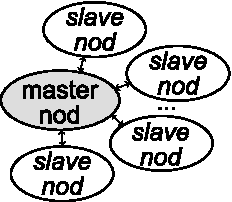
\includegraphics{masterslave.pdf}}
\caption{\label{fig:masterslave}The composition of distributed application}
\end{figure}

Preprocessing of input is another crucial part of algorithm. In situation of discrete logarithm problem it is composed of factorization of value $(p-1)$ that could be afterward used in Pohlig--Hellman algorithm. The computation of the parameters of numerical methods is also important part of this step. It consists of finding of the right composition of each factor base (rational factor base is composed of prime numbers and in situation of GNFS method there is also algebraic factor base with similar composition) and another relevant parameters (for example searching for right value coefficients of polynomial in GNFS method). 

Other important duty of master node is to handle the network communication. It consists of distributing of current task and parameters of numerical methods. Master nod also has to fetch computed values (that are smooth over the given factor base) from slave nods, check them and save them for matrix processing part.

Master nod also use the Montgomery's block Lanczos algorithm for computing of null space of found matrix over  $\mathbb{Z}_2$ field (in case of the integer factorization problem) and Gaussian elimination method over $\mathbb{Z}_{p-1}$ ring (in case of the discrete logarithm problem). After the sequence of computations it also has to check correctness of found results (and skip to some previous step if they are wrong).

Last but not least function of master node is to save found values or represent results in some human readable form.

\subsection{The slave nod}
The most important feature of slave nod is to compute values of the sieving process. This process is slightly different in each numerical methods:
\begin{itemize}
\item \textbf{Quadratic Sieve} method works with factor base of form $\left(\frac{n \mod p}{p} \right)=1$ for each $p \in F$ (where $\left(\frac{a}{p} \right)$ is a Legendre symbol) and computes smooths $x_i$ inversely from $p \in F$ using Tonelli--Shanks algorithm \cite{niven}.

\item \textbf{GNFS} method works with three different factor bases called algebraic factor base (composed of first degree prime ideals in integer pair representation), rational factor base (composed of prime numbers) and quadratic characteristic factor base (for the purpose of checking smoothness) \cite{hoang}. Slave nod compute only values that are smooth over rational and algebraic factor base. Quadratic characteristic values are computed afterward separately.

\item \textbf{Index Calculus} method works with standard factor base composed of prime numbers. \cite{yan}

\end{itemize}

This process require the fast generator of random numbers and also some fast algorithm for computing reminder after dividing of given random number and the prime number in factor base. Another important feature of algorithm is effective working with large numbers (typically greater than $10^{100}$). 

Another important feature of slave nod is to periodically fetching commands from master nod and sending results back to master nod.



%Kontroluje zadání
%U diskretniho logaritmu zcheckene Pohling-Helmana
%Spočítá parametry numerických metod
%Zašle parametry a zadání slavům
%Řídí veškerou komunikaci
%Počítá operace s maticemi

\section{The FPGA approach}
The suitable way for implementation of the slave nod is to use Zynq-7000 SoC. It contains ARM--based processor with programmable FPGA \cite{zynq}. Program running on processor implements the interface for communication with master nod and also manage custom IP cores' properties. The IP cores created on FPGA implements the functionality relevant for selected method. There are following relevant IP cores in the system:
\begin{itemize}
\item \textbf{Random number generator IP} that generates relevant random numbers and also check its properties (for example GNFS method operates with two coprime numbers, other methods operates with one random integer in some interval). 
\item \textbf{Rational smoothness checking IP} that check whether given integer is smooth over some factor base consists of integers (rational factor base in GNFS method).
\item \textbf{Algebraic smoothness checking IP} that check whether given input is smooth over some algebraic factor base (only GNFS operate with this concept).
\end{itemize}

\begin{figure}[htbp]
\centerline{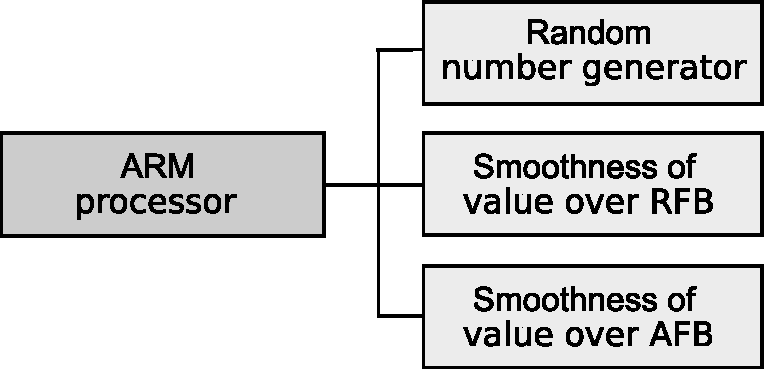
\includegraphics[scale=0.5]{processor.pdf}}
\caption{\label{fig:PROC}Scheme of IP cores of the Zynq system}
\end{figure}

Scheme on the picture \eqref{fig:PROC} is simplified. Many other cores are practically used in the system (for example the core for ethernet communication). 

The Rational smoothness checking on FPGA has been a subject of many improvements \cite{meulenaer}. There is a possibility of checking whether given input is $k$-smooth for some relatively small integer $k$ using Elliptic Curve Method that has already been implemented on FPGA.
%Sekce generovani nahodnych cisel
%Sekce kontroly hladkosti nad faktorovou zakladnou
%



\section{Results of measurement}
After an implementation of distributed system the measurement of its features has been done.% It was especially important to measure the dependency of the average time required for solving of the task to the bit size of input (the presumption is that it has almost exponential character). Another important characteristic is the dependency of the average time required for solving of the task to number of nods (slaves) in the network.

\subsection{Integer factorization problem}
It could be presumed that the dependency of numbers of nods (slaves) in the system and the time required for solving of the task is approximately $\frac{T_0}{S}$ where $T_0$ is time required by single nod and $S$ is the number of nods connected to the system. By using of exponential regression following pattern for computing of $T_0$ has been found:
\begin{equation}
T_0 = 0.31 \cdot 10^{-3} \cdot \exp \left( 0,05 \cdot N \right)
\end{equation}
where $N$ represents bit size of the input ($T_0$ in seconds). Measured results are shown in graph \ref{fig:RSA} bellow.


\begin{figure}[htbp]
\centerline{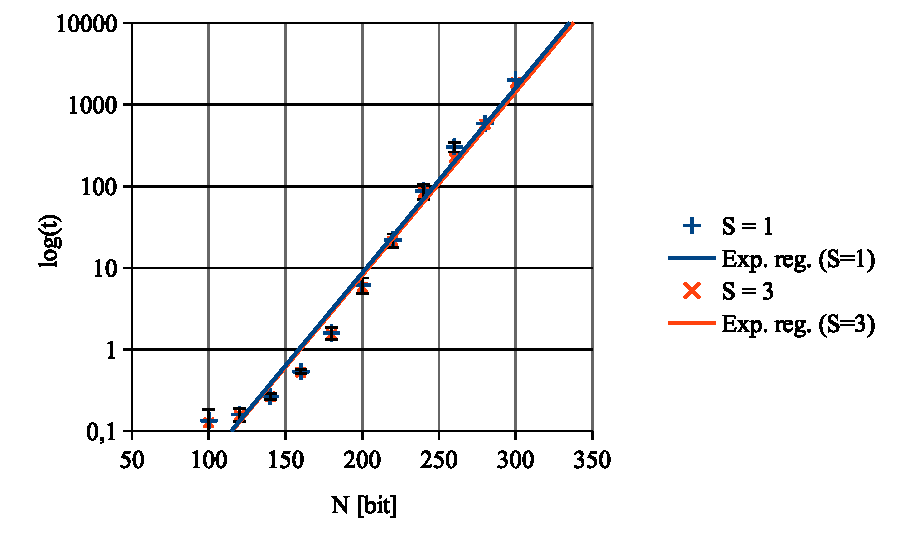
\includegraphics[scale=0.5]{RSA1.pdf} \vspace{-10pt}}
\caption{\label{fig:RSA}Dependency of time to bit size of input (integer factorization problem)}
\end{figure}

The presumption of dependency of numbers of nods (slaves) in the system and the time required for solving of the task has also been confirmed ($t=\frac{T_0}{S}$).

\subsection{Discrete logarithm problem}
Methods for solving of discrete logarithm problem are less effective than the methods for solving of integer factorization problem. This leads to working with input of size smaller than previous measurements works with. Presumptions are exactly same as above.

\begin{figure}[htbp]
\centerline{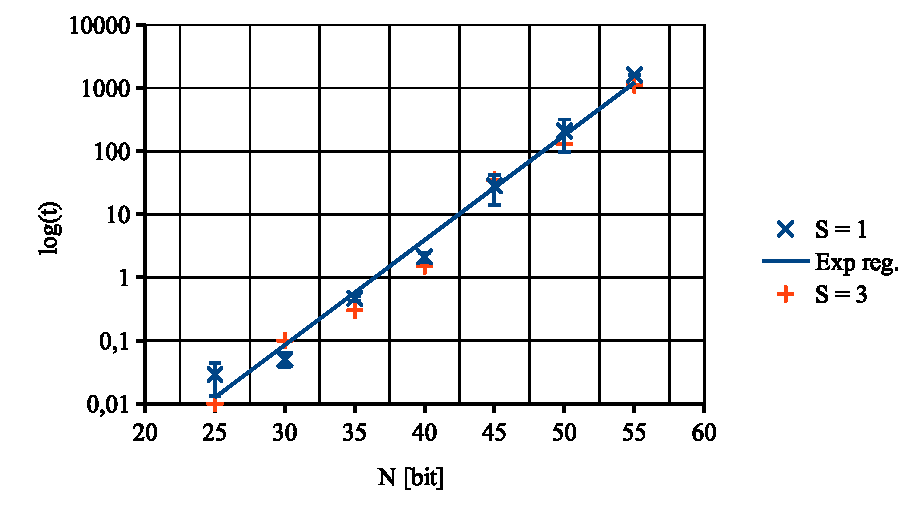
\includegraphics[scale=0.5]{DH1.pdf} \vspace{-10pt}}
\caption{\label{fig:DH}Dependency of time to bit size of input (discrete logarithm problem)}
\end{figure}

Exponential regression of measured values returns following result:
\begin{equation}
T_0 = 8.85 \cdot 10^{-7} \cdot \exp \left( 0.38 \cdot N \right)
\end{equation}
where $N$ represents bit size of the input ($T_0$ in seconds). Measured results are shown in graph \ref{fig:DH}. Presumption of dependency of numbers of nods (slaves) in the system and the time required for solving of the task has also been confirmed as $t=\frac{T_0}{S}$.


\section{Conclusions}% and future research}
This paper represents the possibilities of Zynq-7000 SoC in the cryptanalysis of integer factorization problem and discrete logarithm problem based cryptosystems. It has been shown that using of custom IP cores could accelerate so called sieving part of modern numeric methods for solving of these problems. The sieving unit (or the slave nod of distributed system) is composed of four major parts, the random number generator IP, the IP for checking of smoothness over rational factor base and algebraic factor base and the ARM processor for managing of the process. Paper also discussed the possibilities of parallel approach in this process and also other improvements of used numerical methods for solving of integer factorization and discrete logarithm. The measurement shown that the relation between bit size of input and the time for sieving is almost exponential (that has been presumed) and the relation between number of nods in the system and time spent for sieving is linear (that also has been presumed).

%There exists also many others improvements for selected numerical methods (not only in the way of its implementation). This could be a subject of further research.

%\newpage

\begin{thebibliography}{00}

\bibitem{zynq} L. H. Crockett, R. A. Elliot, M. A. Enderwitz and R. W. Stewart, \textit{The Zynq Book},
Strathclyde Academic Media, 2014, pp. 1-46.
ISBN: 978-0992978709

\bibitem{delfs} H. Delfs and H. Knebl, \textit{Introduction to Cryptography}, 3rd ed. 
Springer, Berlin, Heidelberg, 2015, pp. 49-112.
doi: 10.1007/978-3-662-47974-2

\bibitem{hoang} V. P. Hoang, \textit{Integer factorization with the general number field sieve},
Rovaniemi University of Applied Sciences, 2008, pp. 39-58.
ISBN: 978-952-5153-78-1

\bibitem{meulenaer} G. d. Meulenaer, F. Gosset, G. M. d. Dormale and J. J. Quisquater, "Integer Factorization Based on Elliptic Curve Method: Towards Better Exploitation of Reconfigurable Hardware", %15th Annual IEEE Symposium on Field-Programmable Custom Computing Machines (FCCM 2007), Napa, CA, 2007, pp. 197-206. 
doi: 10.1109/FCCM.2007.12

\bibitem{nguyen} P. Nguyen, "A Montgomery-like square root for the Number Field Sieve", Buhler J.P. (eds) Algorithmic Number Theory. \textit{ANTS 1998}. Lecture Notes in Computer Science, Vol. 1423. Springer, Berlin, Heidelberg

\bibitem{niven} I. Niven, \textit{An Introduction to the Theory of Numbers}, 5th ed.
Wiley, 1991, pp. 110-115.
ISBN: 0-471-62546-9

\bibitem{gireesh} G. Pandey and S. K. Pal, "Polynomial selection in number field sieve for integer factorization", \textit{Perspectives in Science}, Vol. 8, 2016, pp. 101-103, 
doi: 10.1016/j.pisc.2016.04.007.

\bibitem{yan} Y. Y. Song, 2017, \textit{Computational Number Theory and Modern Cryptography},
Higher Education Press, 2017, pp. 191-260.
doi: 10.1002/9781118188606.ch5

\bibitem{lanczos} L. T. Yang, Ying Huang, J. Feng, Q. Pan and C. Zhu, "An improved parallel block Lanczos algorithm over GF(2) for integer factorization", \textit{Information Sciences}, %Vol. 379, 2017, pp. 257-273, 
doi: 10.1016/j.ins.2016.09.052.

\bibitem{wiedemann} L. T. Yang, G. Huang, J. Feng and L. Xu, "Parallel GNFS algorithm integrated with parallel block Wiedemann algorithm for RSA security in cloud computing", \textit{Information Sciences}, %Vol. 387, 2017, pp. 254-265, 
doi: 10.1016/j.ins.2016.10.017.


%PRUMER JE 12 REFERENCI (SPOCTENO ZE SBORNIKU Z LONSKA), MINIMUM AKCEPTOVANEHO CLANKU BYLO 5 REFERENCI



% ----- REFERENCE DLE MUSTRU VYGENEROVANEHO NA SPRINGER.COM ------
%\bibitem{viet} PHAM HOANG VIET. Integer factorization with the general number field sieve: thesis [online]. Rovaniemi: Rovaniemi University of Applied Sciences, 2008 [cit. 2018-01-12]. ISBN 978-952-5153-774.
%\bibitem{wiedemann} Laurence T. Yang, Gaoyuan Huang, Jun Feng, Li Xu, Parallel GNFS algorithm integrated with parallel block Wiedemann algorithm for RSA security in cloud computing, Information Sciences, Volume 387, 2017, Pages 254-265, ISSN 0020-0255, https://doi.org/10.1016/j.ins.2016.10.017.
%\bibitem{lanczos} Laurence T. Yang, Ying Huang, Jun Feng, Qiwen Pan, Chunsheng Zhu, An improved parallel block Lanczos algorithm over GF(2) for integer factorization, Information Sciences, Volume 379, 2017, Pages 257-273, ISSN 0020-0255, https://doi.org/10.1016/j.ins.2016.09.052.
%\bibitem{gireesh} Gireesh Pandey, S.K. Pal, Polynomial selection in number field sieve for integer factorization, Perspectives in Science, Volume 8, 2016, Pages 101-103, ISSN 2213-0209, https://doi.org/10.1016/j.pisc.2016.04.007.
%\bibitem{nguyen} Nguyen P. (1998) A Montgomery-like square root for the Number Field Sieve. In: Buhler J.P. (eds) Algorithmic Number Theory. ANTS 1998. Lecture Notes in Computer Science, vol 1423. Springer, Berlin, Heidelberg
% ------------------

\end{thebibliography}

\end{document}
